\chapter{GPU Implementation}
\label{chap:imp}

Conventional CPU-based parallel Monte Carlo algorithms typically use the approach of one particle history per CPU thread.  Data is accessed when needed and threads execute completely independently of each other.  This is a task-parallel approach, the typical algorithm for which is shown in Figure 1, and works well on CPUs due to their large cache and control sizes (relative to cores) and the lower latency of accessing global memory (smaller penalty for random access).  This approach has been historically called history-based parallelism as well.  To fully utilize the computational power of GPUs, this approach must be modified.  Since all threads in a GPU thread block must execute the same instructions, having conditional statements based on random numbers can cause threads to be serialized, leading to resource under-utilization.  If threads need to execute identical instructions, they therefore must be in the same stage of the transport algorithm.  For example, in particle transport where a particle history is assigned to each thread, thread divergence mainly arises through particles undergoing different reactions based on the results of cross-section sampling.    Studies have been done trying to directly port task-parallel Monte Carlo algorithms to GPUs with some success, most notably that of Liu, et. al. \cite{tianyu}, and they suggest that a data-parallel approach similar to those used in vector computers should be employed \cite{tianyu,vector}.  This approach is also called event-based parallelism since events, such as scattering or surface crossing, are done in parallel for many particles at once.  

Figure 2 shows the data parallel algorithm used to maintain thread coherence (i.e. executing the same instructions) between GPU threads.  It is similar to the vectorized approach used with the early vector computers, which also were able to use a single-instruction, multiple-data (SIMD) execution model \cite{vector,vujic_vector}.  The two main features of Figure 2 are that independent GPU kernel launches are used for each step of the transport chain and that the kernels operate on a large set of particle data (as opposed to transporting one particle at a time).  By doing this, the transport cycle is broken into steps in which a single task, such as determining reaction type or finding boundary intersection, is performed across large dataset of particles and threads can be kept more coherent.

\begin{figure}[h!] 
\centering
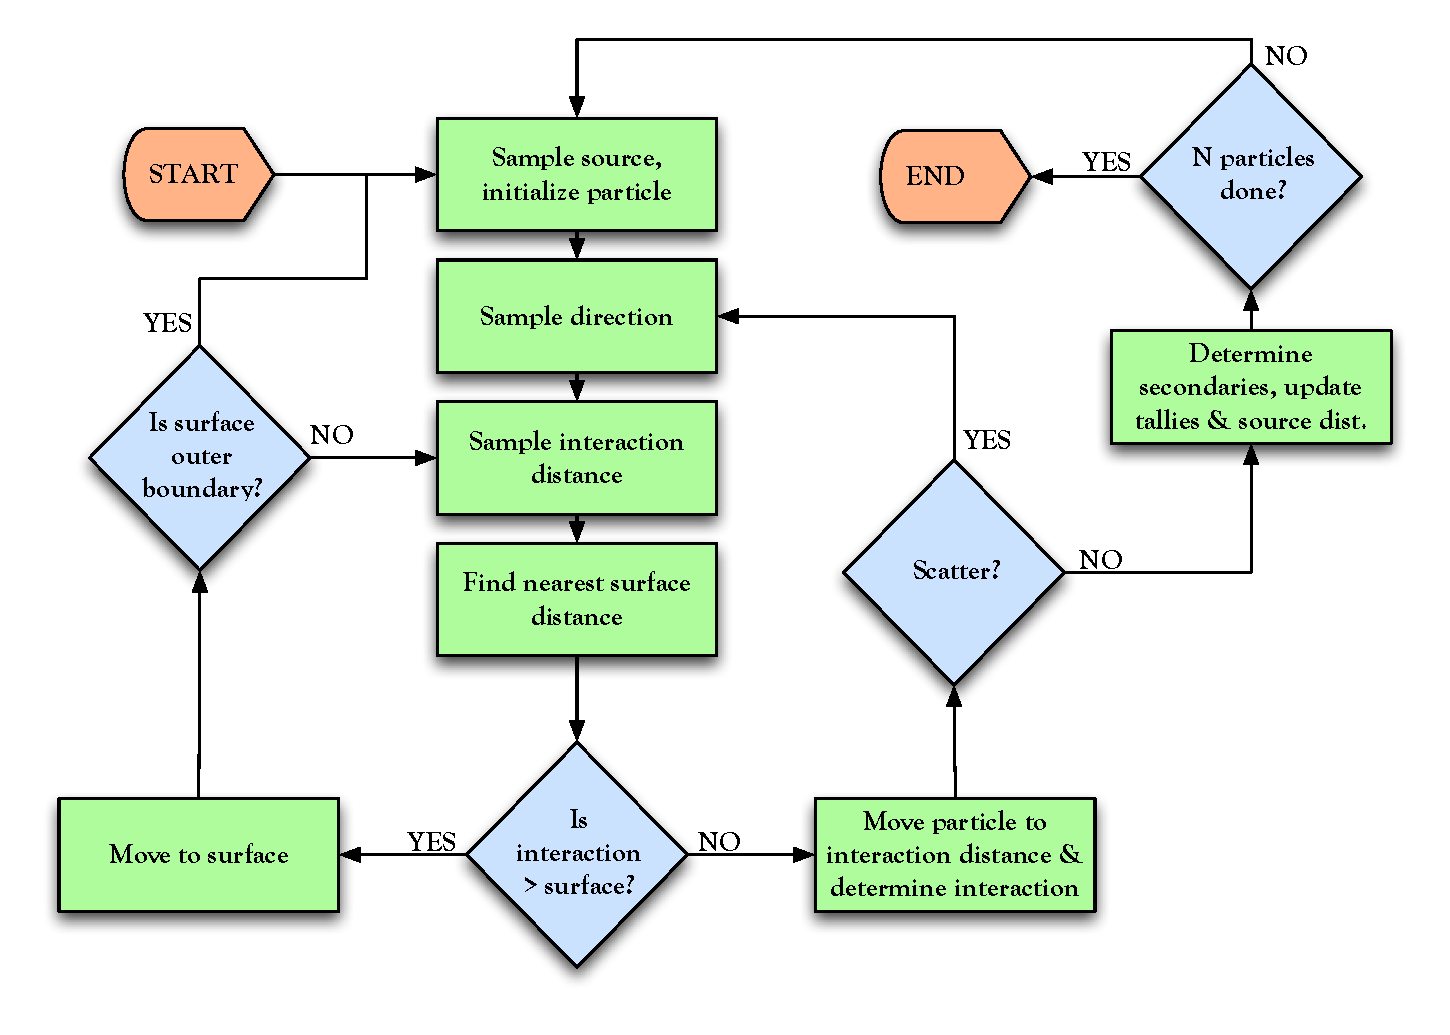
\includegraphics[width=0.8\textwidth]{graphics/task_based_alg.eps}
\caption{Task- or history-based Monte Carlo. \label{task_based_alg} }
\end{figure}

\begin{figure}[h!] 
\centering
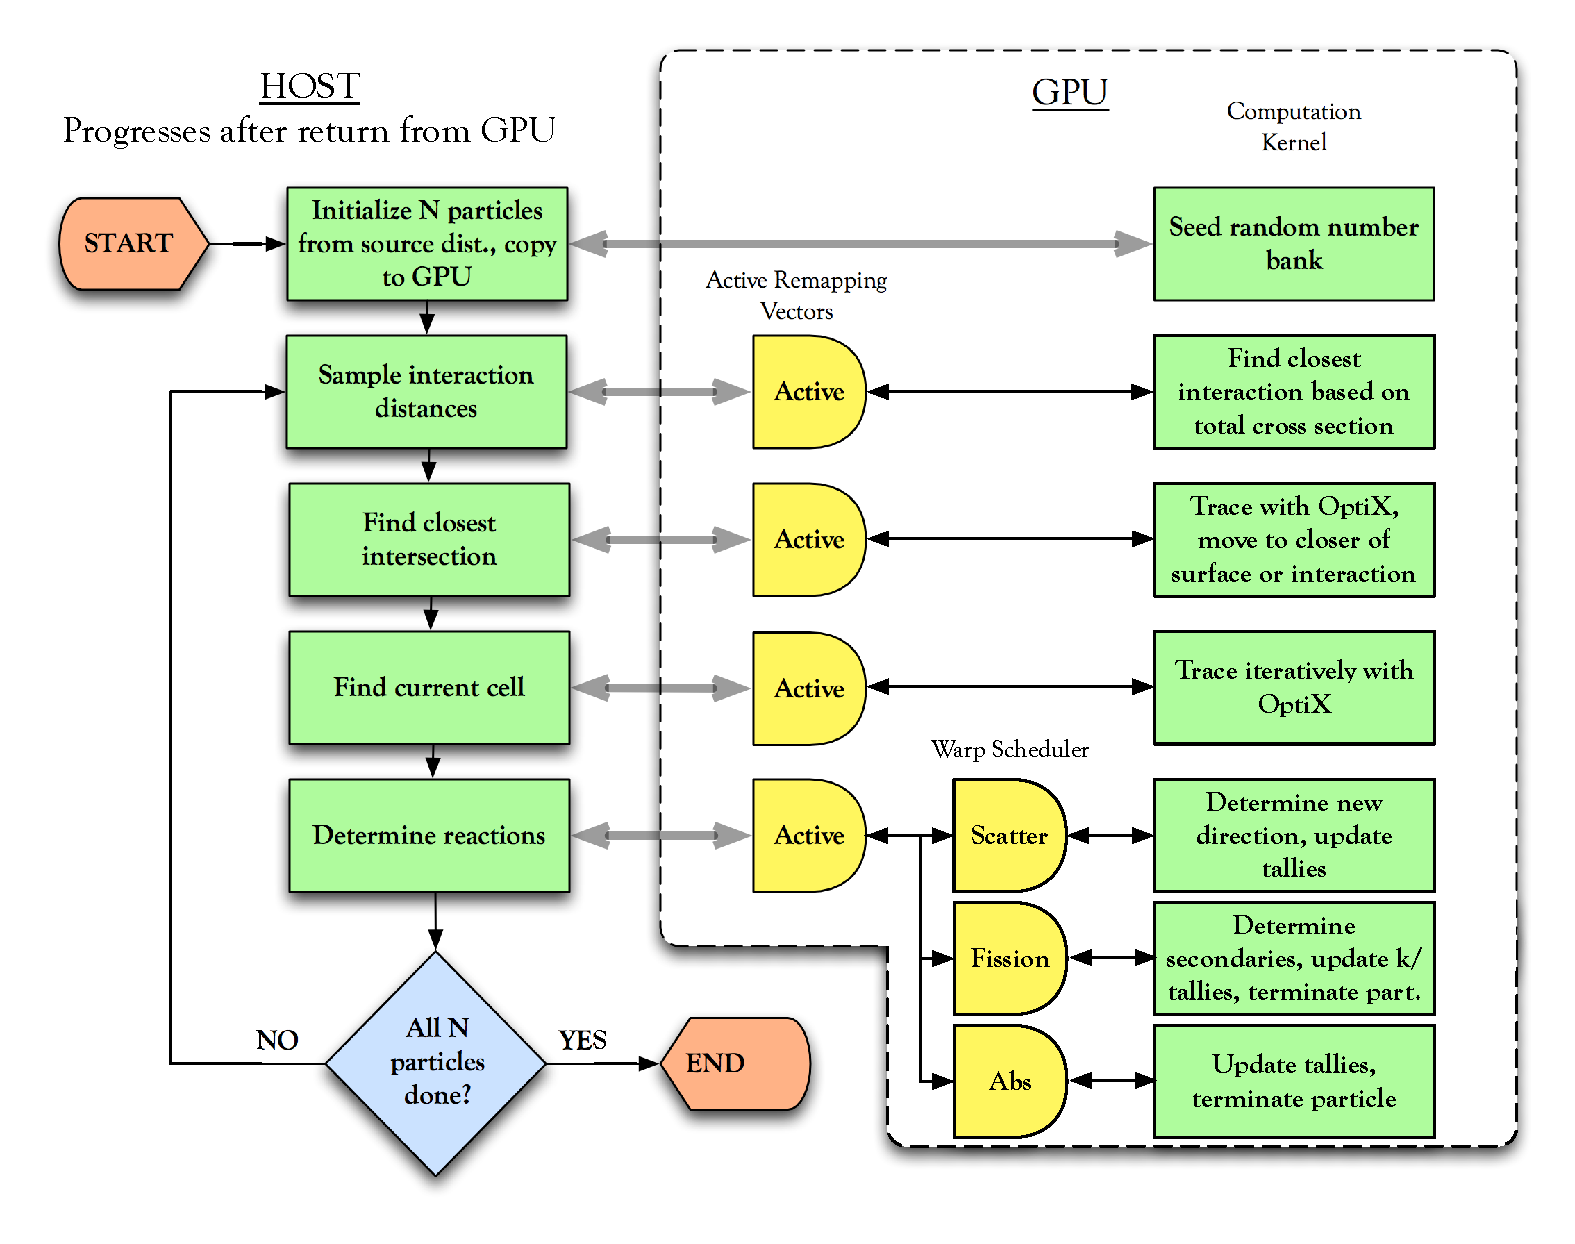
\includegraphics[width=0.8\textwidth]{graphics/event_based_alg.eps}
\caption{Event-based Monte Carlo. \label{event_based_alg} }
\end{figure}


typical task-based MC.  data-parallel MC - wide but single task, homework grading, weaving!

written in C/C++ with some Python, relies on XXX libraries

single vs double precision, justificaiton physics wise and of course cost and performance wise.

%%%%%%%%%%%%%%%%%%%%%%%%%%%%%%

\section{Data Layout}

brief introduction, not using S(a,b) or unresolved resonance parameters at this point

\subsubsection{unionized}

unionized glory, why its good and bad \cite{jaakko}.

constant memory, not much improvement according to nelson

\subsubsection{linked lists}

how to resolve the data heterogeny problem without having massive data replication

float4, have to implement, should be relatively easy

\subsection{Embedded Python}

PyNE

amazing Python C API


%%%%%%%%%%%%%%%%%%%%%%%%%%%%%%

\section{Tasks}

breakdown of tasks into sub-tasks, actually going through how data is stored, accessed, etc

\subsection{Grid Search}

binary search here? more logN?  quad tree?

\subsection{Geometry Representation}

stuff about geom and "where am I?"

\subsubsection{OptiX}

details about ray tracing, how a hit program works

\subsubsection{Acceleration Structures}

Importance of logN


\subsubsection{Point-in-Polygon / Gauss's Law / Divergence Thoerem}

Roll the where am I into  trace

cellular geometry as opposed to combinatorial


\subsubsection{Scaling}

geometry instancing performance tests

optix scaling toy problem - need to have very large sets in order to hide overhead


\subsection{Pseudo-Random Numbers}

use of rejection sampling disqualifies precomputation of random number, plus it is very bandwith intensive to do so!

using lcrng keeps global access down and improves performance greatly

\subsection{Macroscopic}

material

\subsection{Microscopic}

nuclide

\subsection{Interactions}

\subsubsection{Scattering}

Rodriguez rotation

\subsubsection{Secondary-Producing}


\subsubsection{Disappearance}


\subsubsection{Concurrent Kernels}

\subsection{Parallel Operations}

CUDPP, reductions, sums, and sorts - sorting by reaction to keep warps full, memory implications

\subsubsection{Fixed source subcritical multiplication}

necessary to be subcritical.

pop can pop source particles in to keep population constant until NPS exceeded...

\subsubsection{Criticality}

cannot simply pop, unless generation number is associated, then data can be generated and post-processed?

does pop work in supercritical?

need to do generations since the source update is generation-dependent, can this be changed?





